\chapter{セルフトリガを用いた応答評価試験}
この章では,セルフトリガを用いた粒子線に対する応答評価試験について述べる.\ref{sec:latency}節で粒子線を用いた応答評価試験のために必要だったLatencyチューニング機能について述べ,そのあとに,\ref{sec:selfsetup}節で評価試験セットアップ,\ref{sec:selfhow}節で手順,\ref{sec:selfconc}節で取得データの結果を示し,\ref{sec:selfsum}節で考察を行なっている.

\section{Latencyチューニング機能の追加}
\label{sec:latency}
この節では,粒子線に対する応答評価のために必要だったLatencyチューニング機能について述べる.
\subsection{YARRにおけるトリガDAQとLatencyの意義}
YARRソフトウェアを用いたデータ取得におけるトリガDAQについて説明する図を図\ref{fig:YARRDAQ}に示す.\par
\begin{figure}[h]
  \centering
  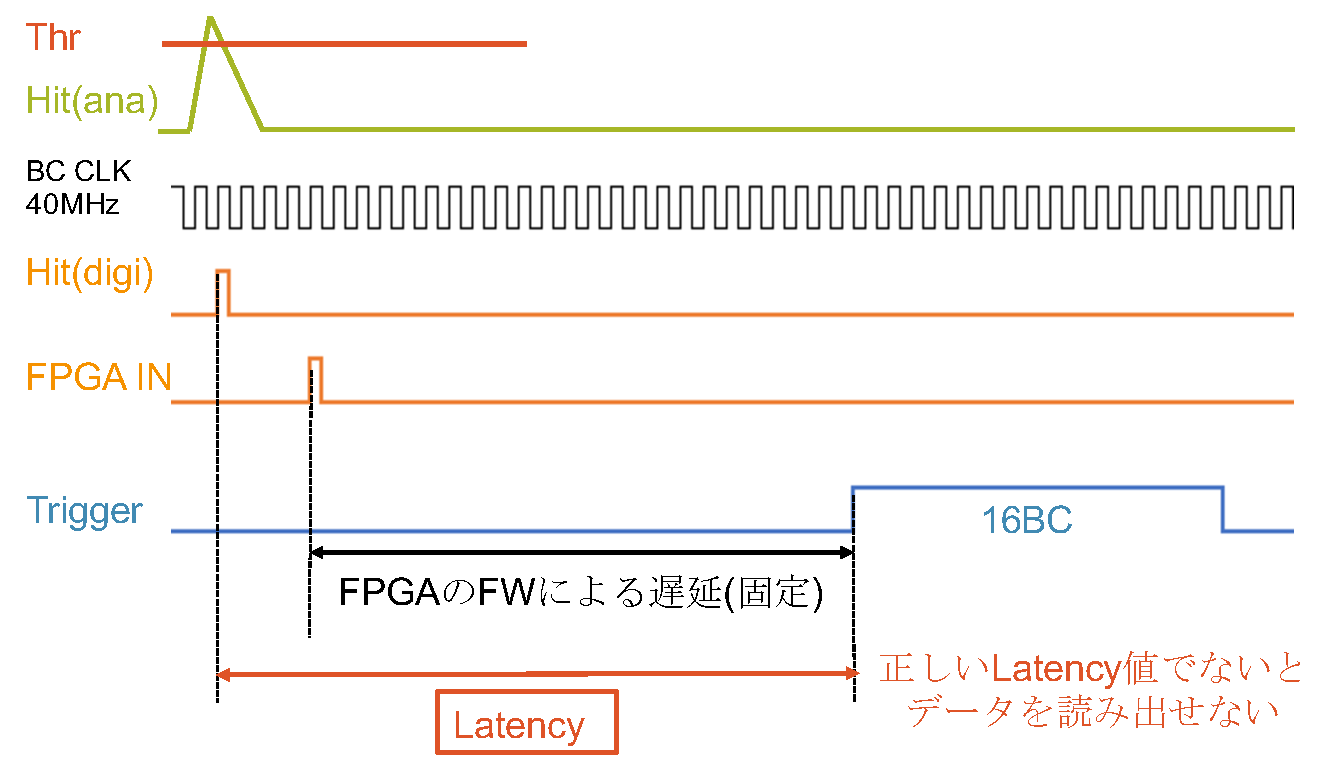
\includegraphics[width=13cm]{./figure/DAQ_signal.pdf}
  \caption{YARRトリガDAQ}
  \label{fig:YARRDAQ}
\end{figure}

Latencyとは,図のtrigger入力時にどれだけの時間遡ってメモリから情報を読み出すかを定める値である.このLatencyがずれていると,データを正しく読み出すことができない.YARRでは,指定されたLatency分遡ったClockの前7 $\mathrm{Clock}$,後8 $\mathrm{Clock}$,計16 $\mathrm{Clock}$分のデータを読み出す.16 $\mathrm{Clock}$の中で何 $\mathrm{Clock}$目のデータであるかを示す値として,L1IDというものが記録される.アナログスキャンにおけるL1IDの分布を以下に示す.\par
\begin{figure}[h]
  \centering
  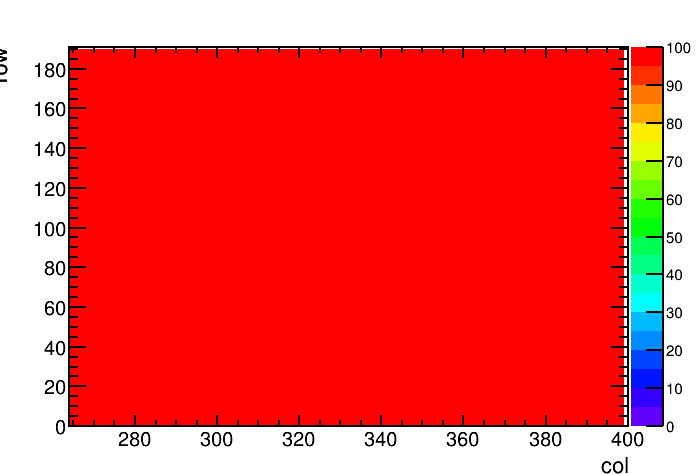
\includegraphics[width=8cm]{./figure/DigitalScan.png}
  \caption{YARRトリガDAQ}
  \label{fig:YARRDAQ}
\end{figure}


理想的にはL1IDが7のところにトリガの中心を合わせたい.そのために,YARRで指定できるLatencyに関する3種類のパラメータを以下に示す.
\subsubsection*{delay1}
FPGAからトリガをどれだけ遅れて出力するかを決める値.本論文では,外部からトリガを受け取ってからどれくらい遅延させてFPGAからRD53Aにトリガを出力するかを決める値.

\subsubsection*{delay2}
擬似パルスを送られてからどれくらい遅れてトリガを出力するかを決める値.前章で述べたデジタルスキャンやアナログスキャンの際に関係し,擬似パルスではなく外部からのトリガを使用してデータ取得するセルフトリガや外部トリガを用いたデータ取得の時には無関係.

\subsubsection*{グローバルレジスタ''LatencyConfig''}
RD53Aの全てのピクセルに共通する設定値であるグローバルレジスタの内の1つにLatencyConfigというLatencyに関する設定値が存在する.LatencyConfigがどのような値であるか説明する図を以下に示す.\par
ASICのあるピクセルが信号を検知すると,そのピクセルが40 $\mathrm{MHz}$のClockに合わせてカウントを始める.そして,FPGAから送られてくるトリガを受け取った時に,そのカウントが設定した''LatencyConfig''の値と等しいピクセルの情報を読み出すようになっている.''LatencyConfig''は,9bitの値であり,0-511まで変化させることが可能である.

\subsection{Latencyチューニング機能}
前節で述べたように,Latencyが合っていないと,データを正しく読み出すことができないので,Latencyを正しい値にすることが,データを正しく読み出す上で大変重要となる.そこで,今回はグローバルレジスタ''LatencyConfig''値を変化させることで,Latencyを合わせられるような機能をYARRに追加した.\par
今回,センサからの信号をASICがHitOR信号として出力したTriggerに対するLatencyを合わせたかった.前章で述べたように,HitOR信号がFPGAに伝わっていることを確認した上で,以下を行なった.
\begin{enumerate}
\item セルフトリガによって100イベントを取得する
\item 取得したデータのL1IDの分布を得る
\item $\mathrm{L1ID} == 7$であるイベント数を記録
\end{enumerate}
以上を0-511の各''LatencyConfig''値に対して行い,''LatencyConfig''値と$\mathrm{L1ID} == 7$だったイベント数の関係を図\ref{fig:latencydist}のように得る.,この時にもっともイベント数が多かった''LatencyConfig''値の時にLatencyが合っていると定義した,

\begin{figure}[h]
  \centering
  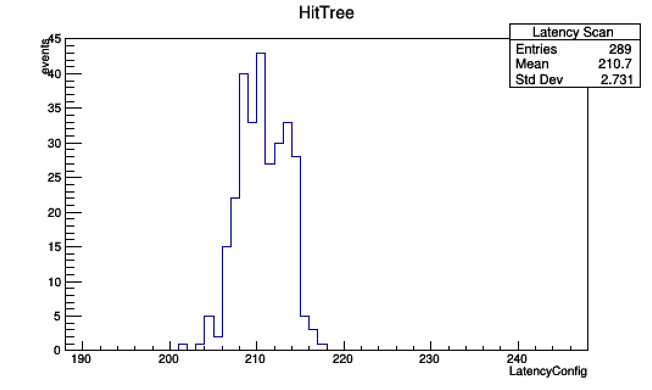
\includegraphics[width=8cm]{./figure/latencydist.png}
  \caption{''LatencyConfig''値とL1ID $== 7$だったイベント数の関係}
  \label{fig:latencydist}
\end{figure}


\subsubsection{Latencyチューニングが幅を持つ理由}
理想的には,Latencyチューニングを行なった時の分布は,正しいLatency値にのみピークが立つはずであるが,今回の結果はそうはなっていない.理由は2つある.
\begin{itemize}
\item YARRの仕組みとして,32bitに1回トリガを発行するかどうかを決めているので,前後8 $\mathrm{Clock}$分の幅が生じる
\item アナログアウトプットのキャパシタンスにズレがあるために前後2 $\mathrm{Clock}$分の幅が生じる.これは,アナログスキャンを行なった時のL1IDの分布を見ると,$\mathrm{L1ID} == 7$のところにのみピークが立つのではなく,前後に2 $\mathrm{Clock}$分の幅を持っていることから確認できる.
\end{itemize}

\section{セルフトリガを用いた応答試験セットアップ}
\label{sec:selfsetup}
主なセットアップは読み出しシステムの動作確認時の図\ref{fig:setup}と変わらず,RD53A搭載のSingle Chip Card(SCC)とFPGAボード,PCを用いて読み出しシステムを構成し,SCCとFPGAボードはアダプタカードを用いてディスプレイポートケーブルによって接続した.センサからの信号を外部に出力するためのコネクタをアダプタカードのport D,RD53Aがコマンドを受け取るためのコネクタをアダプタカードのport Aに繋ぐようにしている.

\section{応答試験手順}
\label{sec:selfhow}
前章で述べたHitOR信号の伝達確認を行なったのち,前節で述べたLatencyチューニングを行った.''LatencyConfig''の分布が図\ref{fig:latencydist}のように得られたため,今回は''LatencyConfig''の値を211に設定することで,Latencyを合わせた.Latencyを合わせた上で,線源を上をセンサに設置した場合としない場合それぞれについて,30分間のセルフトリガによるデータ取得を行なった.

\section{応答試験結果}
\label{sec:selfconc}
図\ref{fig:self}と表\ref{tab:self}に線源をセンサ上に設置した場合としない場合それぞれの,30分間セルフトリガによるデータ取得結果を示す.

\begin{table}[h]
  \centering
  \caption{線源の有無それぞれのヒットレート}
  \begin{tabular} {|l|c|c||c|} \hline
     & \# Hit & 時間[s] & Hitレート[hits/sec] \\  \hline
    線源なし & $3.528 \times 10^6$ & 1800 & 1960 \\ 
    線源あり & $3.599 \times 10^6$ & 1800 & 2000 \\ \hline
  \end{tabular}
  \label{tab:self}
\end{table}

\begin{figure}[h]
  \centering
  \begin{minipage}[b]{0.45\linewidth}
    \centering
    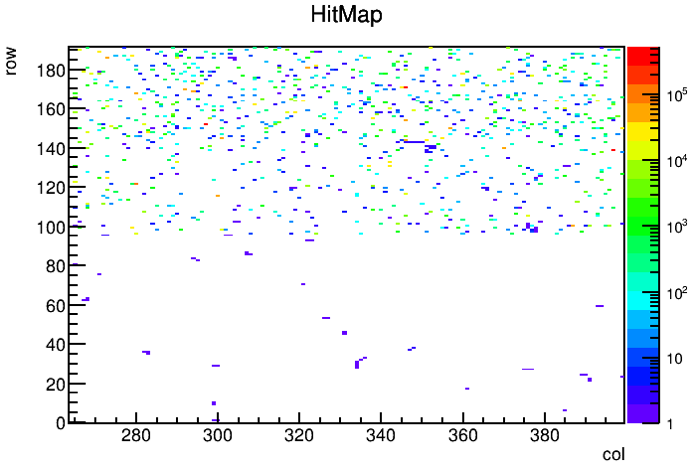
\includegraphics[width=7cm]{./figure/selftrigwo.png}
    \subcaption{線源を置かない場合}
    \label{fig:selfwo}
  \end{minipage}
  \begin{minipage}[b]{0.45\linewidth}
    \centering
    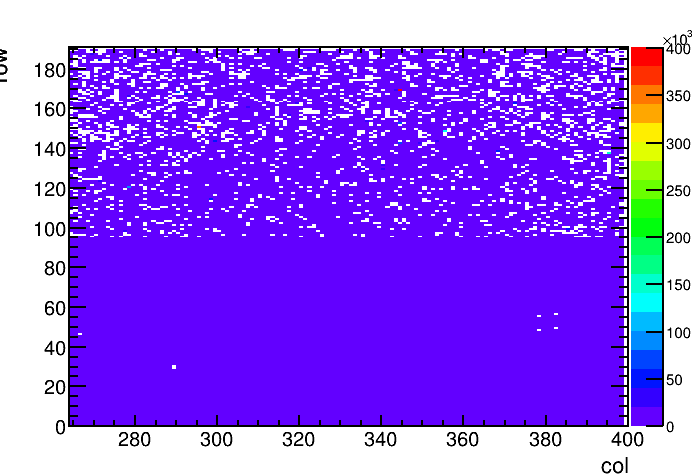
\includegraphics[width=7cm]{./figure/selftrigw.png}
    \subcaption{線源を置いた場合}
    \label{fig:selfo}
  \end{minipage}
  \caption{ヒットの分布}
  \label{fig:self}
\end{figure}

線源あり,なしの場合で,Ocuppancy Mapの分布に差があることが見て取れるが,数値としては,ヒットレートに大きく変化は無かった.応答評価試験として,センサ-ASIC間の接続確認行うためには,センサからの信号でトリガをかけたデータ取得が行われているか確認する必要がある.各ピクセルで線源なし・ありのそれぞれの場合の1ピクセルあたりのHit数分布を図\ref{fig:selfhitfreq}に示す.

\begin{figure}[h]
  \centering
  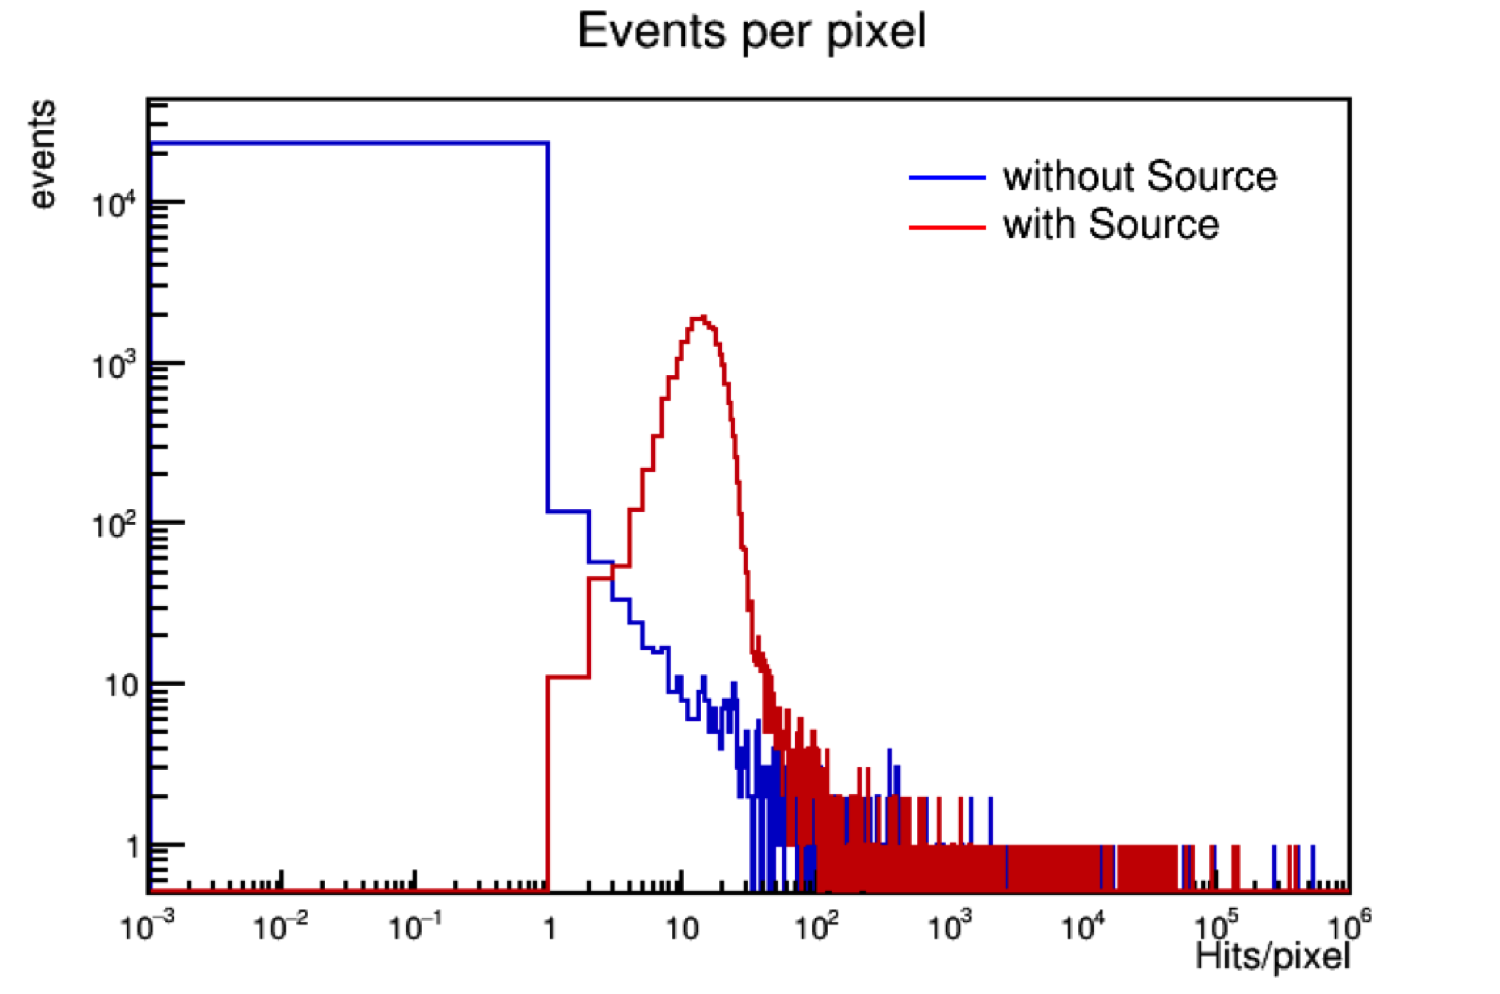
\includegraphics[width=10cm]{./figure/selfhitfreq.png}
  \caption{1ピクセルあたりのHit数分布}
  \label{fig:selfhitfreq}
\end{figure}

このように,線源なしの場合と比較して優位な分布が線源ありの場合に見られる.より詳しく確認するために,以下,線源なしの場合のHit数が0だった場合と,0より大きかった場合に分けて,結果の考察を行なった.

\section{考察}
\label{sec:selfsum}
\subsection*{線源なしの時のHit数が0だった場合}
線源を点線源とみなし,そこから等方的に$\beta$線が放射されていると仮定した場合,今回のセットアップで放射された$\beta$線のうちASICに入射するものの割合を式\ref{eq:beta}を用いて求めた.
\begin{figure}[h]
  \centering
  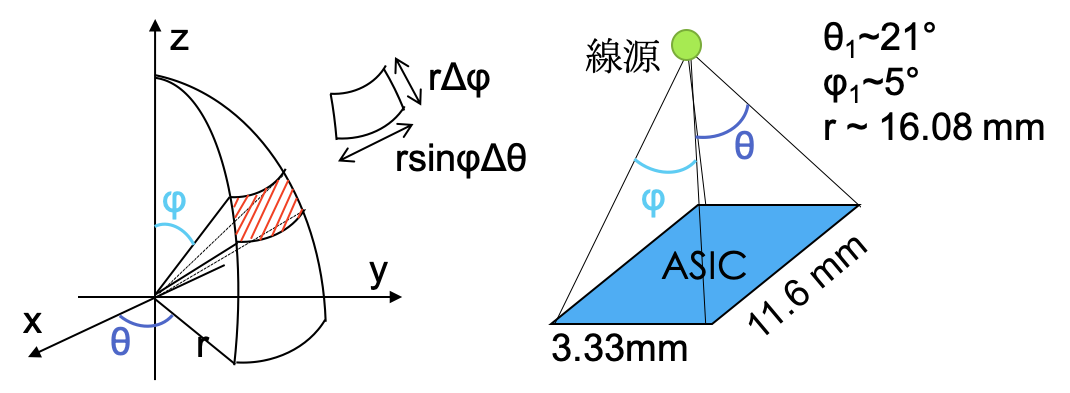
\includegraphics[width=12cm]{./figure/selfarg.png}
  \caption{点線源からの立体角}
\end{figure}

\begin{eqnarray}
  \label{eq:beta}
  \frac{\int^{\phi_1}_0 \int^{\phi_2}_0 r^2 \sin \phi d\theta d\phi}{4 \pi r^2} \simeq 0.28
\end{eqnarray}

本研究で使用したDiff FEのピクセル数が26112,線源の放射能が$4.8 \mathrm{kBq}$であったことから,30分間で1ピクセルが取得できるであろうヒット数を式\ref{eq:hit}のように見積もった.
\begin{eqnarray}
  \label{eq:hit}
  \frac{4.8 \mathrm{kBq} \times 0.28}{26112 \mathrm{pixels}} \times 1800 \mathrm{sec} = 9.18 \mathrm{Hits}
\end{eqnarray}

今回線源からのヒットのデータを取得できていると判断するピクセルの条件を,3ヒットより多くヒットがあったものとした.3ヒットとは,式\ref{eq:hit}より2 $\sigma$の範囲である,$9.18 \times 2 \sqrt{9.18} \simeq 3$から得た値である.線源を置いてデータ取得した場合の1ピクセルあたりのヒット数分布である図\ref{fig:numhitdist}からも,この条件が妥当であることがわかる.この条件を満たし,線源からのヒットがあったと判断したピクセル数を表\ref{tab:0hitdist}に示す.

\begin{figure}[h]
  \centering
  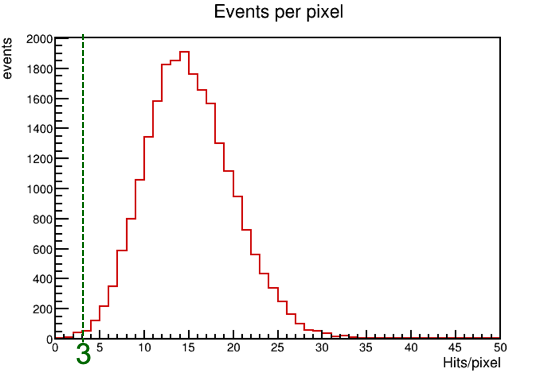
\includegraphics[width=8cm]{./figure/selfperpix.png}
  \caption{線源を置いてデータ取得をした場合の1ピクセルあたりのヒット数}
  \label{fig:numhitdist}
\end{figure}


\begin{table}[h]
  \centering
  \caption{線源からのHitが存在するピクセル数}
  \begin{tabular}{|cl|cl|} \hline
    (i) & 条件を満たすピクセル数 & 22854 & (87.5 \%) \\ \hline
    (ii) & 条件を満たさないピクセル & 56 & (0.2 \%) \\ \hline
  \end{tabular}
  \label{tab:0hitdist}
\end{table}

表\ref{tab:0hitdist}より,30分間のセルフトリガによるデータ取得では,22854個のピクセルが線源からの信号を検出できていると判断できるため,品質保証が可能であることがわかった.一方で,判断できなかった56個のピクセルについては統計量の少なさが原因と考えられるため,今回使用した線源よりも10倍以上強い放射能の線源を用いることで,品質保証が可能になるのではないかと考えた.

\subsection*{線源なしの時のHit数が0より大きかった場合}
